\documentclass{article}

\usepackage[margin=1in]{geometry}
\usepackage{mathtools} %also loads amsmath
\usepackage{amssymb, bbm}
\usepackage[backend=biber,
	style=alphabetic,
	%	citestyle=authoryear,
	natbib=true,
	url=true, 
	doi=true]{biblatex}

%\usepackage{blkarray} % for matrices with labels
\usepackage{microtype}
\usepackage{relsize}
\usepackage{environ}% http://ctan.org/pkg/environ; for capturing body as a parameter for idxmats
\usepackage{tikz}
	\usetikzlibrary{positioning,fit,calc, decorations, arrows, shapes, shapes.geometric}
	\pgfdeclaredecoration{arrows}{draw}{
		\state{draw}[width=\pgfdecoratedinputsegmentlength]{%
			\path [every arrow subpath/.try] \pgfextra{%
				\pgfpathmoveto{\pgfpointdecoratedinputsegmentfirst}%
				\pgfpathlineto{\pgfpointdecoratedinputsegmentlast}%
			};
	}}
	%%%%%%%%%%%%
	
	\tikzset{dpadded/.style={rounded corners=2, inner sep=0.9em, draw, outer sep=0.4em, fill=gray, fill opacity=0.08, text opacity=1}}
	\tikzset{active/.style={fill=blue, fill opacity=0.1}}
	\tikzset{square/.style={regular polygon,regular polygon sides=4, rounded corners = 0}}
	\tikzset{octagon/.style={regular polygon,regular polygon sides=8, rounded corners = 0}}
	
	
	\tikzset{alternative/.style args={#1|#2|#3}{name=#1, circle, fill, inner sep=1pt,label={[name={lab-#1},gray!30!black]#3:\scriptsize #2}} }
	
	
	\tikzset{bpt/.style args={#1|#2}{alternative={#1|#2|above}} }
	\tikzset{tpt/.style args={#1|#2}{alternative={#1|#2|below}} }
	\tikzset{pt/.style args={#1}{alternative={#1|#1|above}} }
	

	\tikzset{mpt/.style args={#1|#2}{name=#1, circle, fill, inner sep=1pt,label={[name={lab-#1},gray]\scriptsize #2}} }
	\tikzset{pt/.style args={#1}{name=#1, circle, fill, inner sep=1pt,label={[name={lab-#1},gray]\scriptsize #1}} }
	
		
		 %\foreach \x in {#1}{(\x) (lab-\x) } 
		 
	\tikzset{Dom/.style args={#1 (#2) around #3}{dpadded, name=#2, label={[name={lab-#2}] #1}, fit={ #3 } }}
	\tikzset{Dom/.style args={#1 (#2) around #3}{dpadded, name=#2, label={[name={lab-#2}] #1}, fit={ #3 } }}
	\tikzset{bDom/.style args={#1 (#2) around #3}{dpadded, name=#2, label={[name={lab-#2}]below:#1}, fit={ #3 } }}
	\tikzset{arr/.style={draw, ->, thick, shorten <=3pt, shorten >=3pt}}
	\tikzset{archain/.style args={#1}{arr, every arrow subpath/.style={draw,arr, #1}, decoration=arrows, decorate}}
	%\tikzset{every label/.append style={text=red, font=\scriptsize}}
	
%	\newcommand\tikzdom[#1;#2](#3,#4[#5]){
%		\foreach [evaluate=\x as \y using (\x-#2/2)/#5 + #3] \x in {0, 1, ..., #2} {
%			\node[bpt={#1\x | $\n_\x$}] at (\y,#4) {};
%		}
%		\node[Dom={$\sf W$ (W) around \lab{w1}\lab{w3}}] {};
%	}

\usepackage{color}
\definecolor{deepgreen}{rgb}{0,0.5,0}

\usepackage[colorlinks=true, citecolor=deepgreen]{hyperref}


\setlength{\skip\footins}{1cm}
\setlength{\footnotesep}{0.4cm}

\usepackage{parskip}
\usepackage{amsthm, thmtools}
\usepackage{
	nameref,%\nameref
	hyperref,%\autoref
	% n.b. \Autoref is defined by thmtools
	cleveref,% \cref
	% n.b. cleveref after! hyperref
}

\begingroup
\makeatletter
\@for\theoremstyle:=definition,remark,plain\do{%
	\expandafter\g@addto@macro\csname th@\theoremstyle\endcsname{%
		\addtolength\thm@preskip\parskip
	}%
}
\endgroup
\makeatother

\theoremstyle{plain}
\newtheorem{theorem}{Theorem}[section]
\newtheorem{coro}{Corollary}[theorem]
\newtheorem{prop}[theorem]{Proposition}
\newtheorem{lemma}[theorem]{Lemma}
\newtheorem{fact}[theorem]{Fact}
\newtheorem{conj}[theorem]{Conjecture}

\theoremstyle{definition}
\newtheorem{defn}{Definition}[section]
\newtheorem{examplex}{Example}[section]
\newenvironment{example}
	{\pushQED{\qed}\renewcommand{\qedsymbol}{$\triangle$}\examplex}
	{\popQED\endexamplex\vspace{-1em}\rule{1cm}{0.7pt}\vspace{0.5em}}

\theoremstyle{remark}
\newtheorem*{remark}{Remark}

\usepackage{xstring}
\usepackage{enumitem}

%\newcommand\duplicat[1]{\gdef\mylist{}\foreach \x in {#1}{\xdef\mylist{\mylist (\x) (lab-\x) }}\mylist} %% this doesn't work :((
\newcommand\lab[1]{(#1)(lab-#1)}


\newcommand{\todo}[1]{{\color{red}\large\textbf{[todo}: {\normalsize\itshape#1}\textbf{]}}}
\newcommand\geqc{\succcurlyeq}
\newcommand\leqc{\preccurlyeq}
\newcommand\mat[1]{\mathbf #1}
\newcommand{\indi}[1]{\mathbbm{1}_{\left[\vphantom{\big[}#1 \vphantom{\big]}\right]}}
\newcommand\m[1]{\mathbf m_{\mathsf #1}}

\newcommand\recall[1]{ Recall \expandarg\cref{rex:#1}:\vspace{-1em} \begingroup\small\color{gray!80!black}\begin{quotation} \expandafter\csname rex:#1\endcsname* \end{quotation}\endgroup }

%OMG THIS WORKS

\def\wrapwith#1[#2;#3]{
	\expandafter#2{\expandarg\StrBefore{#1}{,}}
	\expandarg\StrBehind{#1}{,}[\tmp] 
	\xdef\tmp{\expandafter\unexpanded\expandafter{\tmp}}
	#3
	\expandarg\IfSubStr{\tmp}{,}{\wrapwith{\tmp}[#2;{#3}]}{ \expandafter#2{\tmp} }
}
\def\hwrapcells#1[#2]{\wrapwith#1[#2;&]}
\def\vwrapcells#1[#2]{\wrapwith#1[#2;\\]}



\newsavebox{\idxmatsavebox}
\def\makeinvisibleidxstyle#1#2{\phantom{\hbox{#1#2}}}
\newenvironment{idxmat}[3][\footnotesize\color{gray}\text]{%
	\def\idxstyle{#1}
	\def\colitems{#3}
	\def\rowitems{#2}
	\begin{lrbox}{\idxmatsavebox}$
	\begin{matrix}  \begin{matrix} \hwrapcells{\colitems}[\idxstyle]  \end{matrix} \\[0.1em]
		\left[ 
		\begin{matrix}
			\hwrapcells{\colitems}[\expandafter\makeinvisibleidxstyle\idxstyle]  \\[-1em]
	}{
		\end{matrix}\right]		&\hspace{-0.5em}\begin{matrix*}[l] \vwrapcells{\rowitems}[\idxstyle] \end{matrix*}
	\end{matrix}
	$\end{lrbox}
	\raisebox{0.75em}{\usebox\idxmatsavebox}
%	\vspace{-0.5em}
}

\newenvironment{sqidxmat}[2][\footnotesize\color{gray}\text]
	{\begingroup\idxmat[#1]{#2}{#2}}
	{\endidxmat\endgroup}

\usepackage{ wasysym }

\addbibresource{../refs.bib}
\addbibresource{../maths.bib}


\newcommand{\mfem}{\mathclap\female\male}
\newsavebox{\hourglassbox}
\savebox{\hourglassbox}{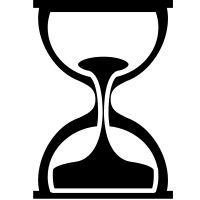
\includegraphics[height=.8em]{hourglass.png}}
\newcommand\hourglass{\usebox{\hourglassbox}}

\newcommand\modelname{{\color{blue!50!black}$\langle$\itshape model name$\rangle$ }}

\title{Discussion of \todo{need name for model} Semantics and Consistency}
\author{Oliver Richardson  \texttt{oli@cs.cornell.edu}}


\begin{document}
	\maketitle

%	\section{The problem with expressing impact as conditional probability.}
%	
%	When we say we have a domain of ``goodness'' $\sf U$, and a conditional probability distribution $\Pr(U \mid A)$, we are not expressing the goodness of $A$, rather estimating the goodness of the world where $A$ takes on various values. This is obviously a belief, and does not work as an expected utility calculation.  How to fix?
%	
%	\subsection{Add more nodes: a separate node for each component}
%	\subsection{Change impact arrows to be functions.}


%	Suppose that we have a diagram
%	
%	\begin{tikzpicture}
%		\node[dpadded](X){$X$};
%		\node[dpadded](A) at (-1, -1.3) {$A$};
%		\node[dpadded](B) at (1, -1.3) {$B$};
%		\node[dpadded](U) at (0, -2.6) {$U$};
%	\end{tikzpicture}

%	Goal: learn preferences over variables, which changes as slowly as possible, to be used in prediction. The classical picture of decision theory is a limit point with infinite cognitive power. You have to coordinate the different levels of preferences, and be very careful to avoid conflicts. 

%	\section{A Defense of  Semantics.}
	Recall that we have a model of nodes, chained together with Markov kernels / conditional probability distributions / stochastic matrices. Of course, there is already an enormous literature about diagrams which look somewhat like this, made up of nodes and conditional probability tables: Baysian Networks (BNs) and their many variants. The diagrams that we employ look very similar, but are intended for a different purpose, and hence have a different semantics. Whereas BN's are a factorization of a particular joint probability distribution and consistent by design, these models are merely constraints on the distribution, which might be so strong so as not to admit any joint distribution.
	
	We will go into the difference more carefully in the next section, but first here are some reasons to prefer this as a way of modeling agents,% in the order of explanation rather than importance:
	
	\begin{enumerate}[nosep]
		\item This representation more naturally matches what humans are aware of, encoding small locally consistent models rather than one giant probability distribution (see sections \ref{sec:human-belief-marginals},\ref{sec:human-pref-marginals})
		\item It is cleaner from a mathematical standpoint: utilities and probabilities are related, we get a notion of belief composition, and we can make use of both category and information theory (sections \ref{sec:util-prob-relate}, \ref{sec:composition}, and \ref{sec:belief-typing}).
		\item This allows composition of arrows to be defined, and gives meanings to paths (section \ref{sec:composition}).
		\item When bits of these diagrams are added and removed, the meaning and form of the rest of the diagram remains the same (section \ref{sec:diagram-alterations}).
		\item We can now represent inconsistency, which we will use to drive preference change. While we agree with the classical picture in that inconsistency is bad, now we can talk about it
		\item Due to the compositionality, it is possible to add typing rules to dynamically change beliefs, knowledge representations, and so forth (section \ref{sec:belief-typing})
		\item It is a strictly more general representation--- we can easily convert BNs to these diagrams (section \ref{sec:convert2bn})
	\end{enumerate}

	
	
	
	\section{Defense of \modelname as a Static Representation }

	
	% Motivating example: why do we need A x B?  Why not just have a BN?
	%	If $A$ and $B$ are random variables, 
	
	
	
	
	
	\subsection{Converting BNs}

	
	% The BN makes the assumption that the value of $D$ cannot depend on anything else; we're only 
%	This also illustrates another important point: the assumptions that you make to drawn a BN, even if locally sensible, build on one another and might not end up being what you wanted to model. On the left it visually looks like you can estimate $D$ from
	% $B$, which is false. It also looks like you can estimate $D$ from 
%	$A$ --- which is true, but only if we've actually modeled all of the confounding factors! For instance, if $B$ has some small mostly negligible dependence on $C$ that we've failed to model, the estimation of $D$ can be arbitrarily bad, if it is sensitive to the correlation between $B$ and $C$.
	





		
	\subsection{Altering Diagrams} \label{sec:diagram-alterations}
	
	\subsection{Relations between Utilities and Probabilities} \label{sec:util-prob-relate}
	\todo{This is in the other documents. I can lift it if this becomes something more stable and we want it here}
	

	
	\section{Inconsistency}
	We will now show how they correspond to other intuitions of inconsistent preferences through some examples and specific cases.
	
	
%	\subsection{Examples of Inconsistency}




	
	\subsection{Learning Problems}
	\todo{adapt from previous document. Most everything there is correct, but in context it doesn't flow. I don't think I got feedback on that section yet}
	
	\section{Dynamics}
	
	Although this looks like a complicated formula full of arbitrary symbols, it is in fact just the minimum total information needed to encode a distribution given your current beliefs. Note that if there is a distribution $p$ that marginalizes out to match each link $L$, then the KL divergence will be zero for each link and input, and therefore the inconsistency will be zero; thus this is a special case of our previous definition.
	
	Although it is not obviously differentiable, this function at least admits sub-gradients, which is a place to look in order to implement gradient descent. One can always also estimate a gradient by sampling, and $\zeta$ is at least continuous.
	
	\subsection{Belief Revision}
	

	
	\subsection{Preference Thermodynamics} \label{sec:thermo}
	We now have a quantity that behaves like enthalpy (inconsistency, $\zeta$), as well as information theoretic entropy. We now ask the question: is it reasonable to use these and a temperature parameter to define an effective free energy for belief revision?
	
	\[ G := \zeta - T H \]
	

	At low temperatures, $G = \zeta$, so gradient descent is just minimization of inconsistency. At high temperatures, using gradient descent on $G$ is mostly just entropy maximization: this corresponds to a softening of beliefs and preferences. 
	
	Of course, temperature could also be localized more to some links over others: you could be more willing or primed to reconsider beliefs about things you've just learned, for instance. Temperature can therefore function as the entrenchment parameter we've been looking for, and actually fits well with the physical analogy. When things are hot, they're malleable and are easily molded by the environment; as they cool off, they keep their history and identity. This seems like a fitting way of viewing agents as well.
	
	\section{A More Formal Treatment}
	
	We will build up a few intermediate results, and make this discussion more formal, to prove the theorems. First,
	
	\begin{defn}
		A Baysian network (BN) is a tuple
		\[
			\mathcal B = \left(\mathcal N : \mathbf{FinSet}, ~~\mathrm{Par}: \mathcal N \to 2^{\mathcal N},~~ \mathcal S: \mathcal N \to \mathbf{FinSet},~~\Pr: \prod_{N : \mathcal N}  \left[ \mathcal S_N \times \left(\prod_{P : \mathrm{Par}(N)} \mathcal S_P\right)  \to [0,1] \right] \right)
		\]
		such that
		\begin{itemize}[nosep]
			\item the graph $\bigcup_{N, P \in \mathrm{Par}(N)}(N, P)$ is acyclic, i.e., there exists no cycle of nodes $N_0, N_1, \cdots, N_k = N_0$ in $\mathcal N^k$ such that $N_{i+1} \in \mathrm{Par}(N_i)$ for each $i \in \{0, 1, \cdots, k\}$.
			\item For all $N \in \mathcal N$, $\Pr(N)$ is a probability distribution on $\mathcal S_N$, i.e., 
			\[ \forall N\in \mathcal N.~\forall \vec{p} \in {\prod_{P : \mathrm{Par}(N)} \mathcal S_P}.~~ \sum_{n \in \mathcal S_{N}} \Pr_N(\vec{p}, n) = 1\]
		\end{itemize}
	\end{defn}

	A BN represents a factorization of a joint probability on all of its variables $\mathcal N$ into conditional probability tables. Our model is a similar, but weaker:

	\begin{defn}\label{def:mcg}
		A marginal constraint graph is a tuple 
		\[ \left(\mathcal N : \mathbf{FinSet},~~\mathcal L : 2^{\cal N \times N},~~ \langle\mathcal S, \Sigma\rangle : \mathcal N \to \mathbf{MeasSet}, ~~\mathbf p : \prod_{(A,B): \mathcal L} \left[ \Big. \mathcal S_A \times \Sigma_B \to [0,1]\right] \right) \]
		where $p(L)$ is a Markov kernel, i.e., for every $L[A,B] : \mathcal L$, and $a \in \mathcal S_A$, $\mathbf p_L[a \mid \cdot~]$ is a probability distribution on $(\mathcal S_B, \Sigma_B)$, and $\mathbf p_L[~\cdot \mid B]$ is $\Sigma_A$-measurable for every $B \in \Sigma_B$.
	\end{defn}

	
	\begin{defn}
		If $\mathcal B = (\mathcal N, \mathrm{Par}, \mathcal S, \Pr)$ is a Bayesian Network, then let $\Gamma \cal B$ denote the corresponding marginal constraint graph given by the procedure in section \ref{sec:convert2bn}. Explicitly, 
		\[ \Gamma\mathcal B :=  (\mathcal N', \mathcal L, (\mathcal S, \Sigma), \mathbf p) \]
		where % $\mathcal N'$ is the original nodes, plus
		\begin{align*}
			\mathcal N' &=  \left\{ \Big.\{N\} \mid N \in \mathcal N\right\} \cup \left\{ \mathrm{Par}(N) ~\middle|~ N \in \cal N \right\} \\%
			\mathcal L &= \left\{ \vphantom{\Big|}(\mathrm{Par}(N), \{N\}) \mid N \in \mathcal N \right\} \cup 
				\left\{\vphantom{\Big|} (P, \{X\}) \mid X \in P, P = \mathrm{Par}(N) \text{ for some }N \in \mathcal N \right\} \\
			\mathcal S'_N &= \prod_{X \in N} \mathcal S_X \qquad;\qquad
				\Sigma_N = \bigotimes_{X \in N} 2^{\mathcal S_X}, \text{the product algebra of discrete $\sigma$-algebras} \\
			\mathbf p &= \begin{cases}
				 	(\mathrm{Par}(N), \{N\}) &\mapsto \lambda(p, B).~ \displaystyle\sum_{b \in  B} \Pr(b \mid p) \\
				 	(P, X) &\mapsto, \lambda (p, B).~ \displaystyle \mathbbm 1_{\displaystyle\pi_X(p) \in B}
				\end{cases}
		\end{align*}
		%\cpm p(\frac{a}{z}|b)
	\end{defn}
	All we've done is explicitly add parent nodes and projection edges to our graph, plus some formalities with a trivial $\sigma$-algebra so that we can use definition \ref{def:mcg} exactly, which will need to eventually also accommodate continuous variables --- but in this case everything is discrete. We have also subtly (by adding curly braces in the right places and taking unions rather than disjoint unions) eliminated the duplicate nodes arising from edges in the original BN which only have a single parent.

	
%	\begin{lemma}
%		If $\mathcal B = (\mathcal N, \mathrm{Par}, \mathcal S, \Pr)$ is a BN, and $p$ is a distribution on $\mathcal S$ that marginalizes to each of the links in $\Gamma(\mathcal B)$, then for all variables $N \in \mathcal N$, $\Pr(N = n) = p(N=n)$
%	\end{lemma}
%	\begin{proof}
%		content
%	\end{proof}

	\begin{lemma}
		If $A$, $B$, $C$ are variables with a joint distribution $p$, then $H_p(A \mid B, C) \leq H_p(A \mid C)$ with equality if and only if $A \CI B \mid C$.
	\end{lemma}
	\begin{proof}
		We'll start with the inequality. 
		\begin{align*}
			H(A \mid B, C) = H(A,B,C) - H(B,C)
		\end{align*}
		$(\impliedby)$. Suppose that 
	\end{proof}
	
	We will now prove the theorem:
	\begin{theorem}
		If $\mathcal B$ is a BN, with nodes $\cal N$ and states $\cal S$, then the center of $\Gamma\cal B$ is a unique distribution $p$ on $\prod \mathcal S$, equal to $\Pr$, the distribution that $\mathcal B$ represents.
	\end{theorem}
	\begin{proof}
		Since BN's are acyclic and $\cal N$ is finite, there is an ordering of $\mathcal N$ = $X_0, X_1, \cdots$ such that the parents of each node $X_i$ all come before $X_i$ itself. Now, looking at the joint entropy of all of the variables, we have:
		
		\[	H_p(\mathcal N) = H_p(X_0) + H_p(X_1 \mid X_0) + H_p(X_2 \mid X_1, X_0) + \cdots \]
		
		By Lemma \ref{lem:iff} $H(A\mid B) \leq H(A \mid B, C)$
	\end{proof}
		
	
\end{document}